\documentclass[]{book}
\usepackage{lmodern}
\usepackage{amssymb,amsmath}
\usepackage{ifxetex,ifluatex}
\usepackage{fixltx2e} % provides \textsubscript
\ifnum 0\ifxetex 1\fi\ifluatex 1\fi=0 % if pdftex
  \usepackage[T1]{fontenc}
  \usepackage[utf8]{inputenc}
\else % if luatex or xelatex
  \ifxetex
    \usepackage{mathspec}
  \else
    \usepackage{fontspec}
  \fi
  \defaultfontfeatures{Ligatures=TeX,Scale=MatchLowercase}
\fi
% use upquote if available, for straight quotes in verbatim environments
\IfFileExists{upquote.sty}{\usepackage{upquote}}{}
% use microtype if available
\IfFileExists{microtype.sty}{%
\usepackage{microtype}
\UseMicrotypeSet[protrusion]{basicmath} % disable protrusion for tt fonts
}{}
\usepackage[margin=1in]{geometry}
\usepackage{hyperref}
\hypersetup{unicode=true,
            pdftitle={R语言玩转金融与体彩数据分析},
            pdfauthor={®γσ,黄联富},
            pdfborder={0 0 0},
            breaklinks=true}
\urlstyle{same}  % don't use monospace font for urls
\usepackage{natbib}
\bibliographystyle{apalike}
\usepackage{color}
\usepackage{fancyvrb}
\newcommand{\VerbBar}{|}
\newcommand{\VERB}{\Verb[commandchars=\\\{\}]}
\DefineVerbatimEnvironment{Highlighting}{Verbatim}{commandchars=\\\{\}}
% Add ',fontsize=\small' for more characters per line
\usepackage{framed}
\definecolor{shadecolor}{RGB}{248,248,248}
\newenvironment{Shaded}{\begin{snugshade}}{\end{snugshade}}
\newcommand{\AlertTok}[1]{\textcolor[rgb]{0.94,0.16,0.16}{#1}}
\newcommand{\AnnotationTok}[1]{\textcolor[rgb]{0.56,0.35,0.01}{\textbf{\textit{#1}}}}
\newcommand{\AttributeTok}[1]{\textcolor[rgb]{0.77,0.63,0.00}{#1}}
\newcommand{\BaseNTok}[1]{\textcolor[rgb]{0.00,0.00,0.81}{#1}}
\newcommand{\BuiltInTok}[1]{#1}
\newcommand{\CharTok}[1]{\textcolor[rgb]{0.31,0.60,0.02}{#1}}
\newcommand{\CommentTok}[1]{\textcolor[rgb]{0.56,0.35,0.01}{\textit{#1}}}
\newcommand{\CommentVarTok}[1]{\textcolor[rgb]{0.56,0.35,0.01}{\textbf{\textit{#1}}}}
\newcommand{\ConstantTok}[1]{\textcolor[rgb]{0.00,0.00,0.00}{#1}}
\newcommand{\ControlFlowTok}[1]{\textcolor[rgb]{0.13,0.29,0.53}{\textbf{#1}}}
\newcommand{\DataTypeTok}[1]{\textcolor[rgb]{0.13,0.29,0.53}{#1}}
\newcommand{\DecValTok}[1]{\textcolor[rgb]{0.00,0.00,0.81}{#1}}
\newcommand{\DocumentationTok}[1]{\textcolor[rgb]{0.56,0.35,0.01}{\textbf{\textit{#1}}}}
\newcommand{\ErrorTok}[1]{\textcolor[rgb]{0.64,0.00,0.00}{\textbf{#1}}}
\newcommand{\ExtensionTok}[1]{#1}
\newcommand{\FloatTok}[1]{\textcolor[rgb]{0.00,0.00,0.81}{#1}}
\newcommand{\FunctionTok}[1]{\textcolor[rgb]{0.00,0.00,0.00}{#1}}
\newcommand{\ImportTok}[1]{#1}
\newcommand{\InformationTok}[1]{\textcolor[rgb]{0.56,0.35,0.01}{\textbf{\textit{#1}}}}
\newcommand{\KeywordTok}[1]{\textcolor[rgb]{0.13,0.29,0.53}{\textbf{#1}}}
\newcommand{\NormalTok}[1]{#1}
\newcommand{\OperatorTok}[1]{\textcolor[rgb]{0.81,0.36,0.00}{\textbf{#1}}}
\newcommand{\OtherTok}[1]{\textcolor[rgb]{0.56,0.35,0.01}{#1}}
\newcommand{\PreprocessorTok}[1]{\textcolor[rgb]{0.56,0.35,0.01}{\textit{#1}}}
\newcommand{\RegionMarkerTok}[1]{#1}
\newcommand{\SpecialCharTok}[1]{\textcolor[rgb]{0.00,0.00,0.00}{#1}}
\newcommand{\SpecialStringTok}[1]{\textcolor[rgb]{0.31,0.60,0.02}{#1}}
\newcommand{\StringTok}[1]{\textcolor[rgb]{0.31,0.60,0.02}{#1}}
\newcommand{\VariableTok}[1]{\textcolor[rgb]{0.00,0.00,0.00}{#1}}
\newcommand{\VerbatimStringTok}[1]{\textcolor[rgb]{0.31,0.60,0.02}{#1}}
\newcommand{\WarningTok}[1]{\textcolor[rgb]{0.56,0.35,0.01}{\textbf{\textit{#1}}}}
\usepackage{longtable,booktabs}
\usepackage{graphicx,grffile}
\makeatletter
\def\maxwidth{\ifdim\Gin@nat@width>\linewidth\linewidth\else\Gin@nat@width\fi}
\def\maxheight{\ifdim\Gin@nat@height>\textheight\textheight\else\Gin@nat@height\fi}
\makeatother
% Scale images if necessary, so that they will not overflow the page
% margins by default, and it is still possible to overwrite the defaults
% using explicit options in \includegraphics[width, height, ...]{}
\setkeys{Gin}{width=\maxwidth,height=\maxheight,keepaspectratio}
\IfFileExists{parskip.sty}{%
\usepackage{parskip}
}{% else
\setlength{\parindent}{0pt}
\setlength{\parskip}{6pt plus 2pt minus 1pt}
}
\setlength{\emergencystretch}{3em}  % prevent overfull lines
\providecommand{\tightlist}{%
  \setlength{\itemsep}{0pt}\setlength{\parskip}{0pt}}
\setcounter{secnumdepth}{5}
% Redefines (sub)paragraphs to behave more like sections
\ifx\paragraph\undefined\else
\let\oldparagraph\paragraph
\renewcommand{\paragraph}[1]{\oldparagraph{#1}\mbox{}}
\fi
\ifx\subparagraph\undefined\else
\let\oldsubparagraph\subparagraph
\renewcommand{\subparagraph}[1]{\oldsubparagraph{#1}\mbox{}}
\fi

%%% Use protect on footnotes to avoid problems with footnotes in titles
\let\rmarkdownfootnote\footnote%
\def\footnote{\protect\rmarkdownfootnote}

%%% Change title format to be more compact
\usepackage{titling}

% Create subtitle command for use in maketitle
\newcommand{\subtitle}[1]{
  \posttitle{
    \begin{center}\large#1\end{center}
    }
}

\setlength{\droptitle}{-2em}

  \title{R语言玩转金融与体彩数据分析}
    \pretitle{\vspace{\droptitle}\centering\huge}
  \posttitle{\par}
  \subtitle{R语言量化交易}
  \author{\href{https://beta.rstudioconnect.com/content/3091/ryo-eng.html}{®γσ,黄联富}}
    \preauthor{\centering\large\emph}
  \postauthor{\par}
      \predate{\centering\large\emph}
  \postdate{\par}
    \date{2018-09-17}

\usepackage{booktabs}

\usepackage{amsthm}
\newtheorem{theorem}{Theorem}[chapter]
\newtheorem{lemma}{Lemma}[chapter]
\theoremstyle{definition}
\newtheorem{definition}{Definition}[chapter]
\newtheorem{corollary}{Corollary}[chapter]
\newtheorem{proposition}{Proposition}[chapter]
\theoremstyle{definition}
\newtheorem{example}{Example}[chapter]
\theoremstyle{definition}
\newtheorem{exercise}{Exercise}[chapter]
\theoremstyle{remark}
\newtheorem*{remark}{Remark}
\newtheorem*{solution}{Solution}
\begin{document}
\maketitle

{
\setcounter{tocdepth}{1}
\tableofcontents
}
\hypertarget{preface}{%
\chapter{前言}\label{preface}}

\textbf{为何辑写此书}

本书是在下首次辑写参考书(纯属个人经验分享与心得),此前分享了\textbf{如何安装®Studio服务器与Shiny服务器}\footnote{\href{https://github.com/scibrokes/setup-rstudio-server}{安装
  ®StudioとShiny服务器}}:

\begin{itemize}
\tightlist
\item
  \href{https://beta.rstudioconnect.com/englianhu/Introducing-RStudio-Server-for-Data-Scientists/Introducing-RStudio-Server-for-Data-Scientists.html}{为数据科学家们量身定做の专业统计软件
  --- ®Studio服务器}
\item
  \href{https://beta.rstudioconnect.com/englianhu/Introducing-RStudio-Server-for-Data-Scientists-Slides/Introducing-RStudio-Server-for-Data-Scientists-slides.html}{为数据科学家们量身定做の专业统计软件
  --- ®Studio服务器(演示文稿)}
\end{itemize}

在下来自于马来西亚\footnote{个人简历请查阅:\href{https://beta.rstudioconnect.com/content/3091/ryo-eng.html}{®γσ,
  ENG LIAN HU}},自2005年入行体彩交易就学习Excel电子表格,而2008年加入\textbf{Scicom
(MSC)
Bhd}后开始接触R语言,并且活跃于\href{https://d.cosx.org}{统计之都论坛}与\href{http://bbs.pinggu.org/forum-69-1.html}{经管之家:R语言论坛}论坛俩与中国大陆同胞交流,并向前辈高手们学习。

前几年,偶然发现了个R语言的使用者界面\textbf{®Studio}后,就觉得非常方便,然后自学在\href{https://m.do.co/c/aabb124120d0}{DigitalOcean.com}安装服务器方便随时随地,只要可以上网的地方就可以使用。

前阵子,在下在学习金融交易的时候,无意中发现了本非常实用的经验分享书籍\href{https://raw.githubusercontent.com/englianhu/binary.com-interview-question/master/reference/Successful\%20Algorithmic\%20Trading.pdf}{Successful
Algorithmic
Trading},笔者在金融交易的解说,由入门到精通包括编码分享(笔者介绍了R语言、Python、C++以及比较各优缺点),该笔者\textbf{Michael
Halls}\footnote{更多该作者详情,请参阅\href{https://www.quantstart.com/successful-algorithmic-trading-ebook}{Struggling
  To Make Profitable Algo Trading Strategies?}}与在下一样以经验分享著书之见,在下阅读与学习时深深感受到金融交易的武功秘籍(实用教材)如兮,夫复何求哇!

在下才疏学浅,仅有约翰霍金斯大学数据科学专业文凭,倘若有何错误之处,涵清多多包涵并指教。此书乃个人经验之谈。希望在同感身受与共而勉之的情况之下,热衷于金融与体彩行业的学者们可以容易着手。

有关如何辑写\texttt{bookdown::gitbook}网络书籍,请参阅\href{https://bookdown.org/yihui/bookdown/}{bookdown:
Authoring Books and Technical Documents with R Markdown}。

\begin{center}\rule{0.5\linewidth}{\linethickness}\end{center}

\textbf{Powered by - Copyright® Intellectual Property Rights of
\href{http://www.scibrokes.com}{Scibrokes®}個人の経営企業}

\hypertarget{intro}{%
\chapter{介绍}\label{intro}}

You can label chapter and section titles using \texttt{\{\#label\}}
after them, e.g., we can reference Chapter \ref{intro}. If you do not
manually label them, there will be automatic labels anyway, e.g.,
Chapter \ref{methods}.

Figures and tables with captions will be placed in \texttt{figure} and
\texttt{table} environments, respectively.

\begin{Shaded}
\begin{Highlighting}[]
\KeywordTok{par}\NormalTok{(}\DataTypeTok{mar =} \KeywordTok{c}\NormalTok{(}\DecValTok{4}\NormalTok{, }\DecValTok{4}\NormalTok{, }\FloatTok{.1}\NormalTok{, }\FloatTok{.1}\NormalTok{))}
\KeywordTok{plot}\NormalTok{(pressure, }\DataTypeTok{type =} \StringTok{'b'}\NormalTok{, }\DataTypeTok{pch =} \DecValTok{19}\NormalTok{)}
\end{Highlighting}
\end{Shaded}

\begin{figure}

{\centering 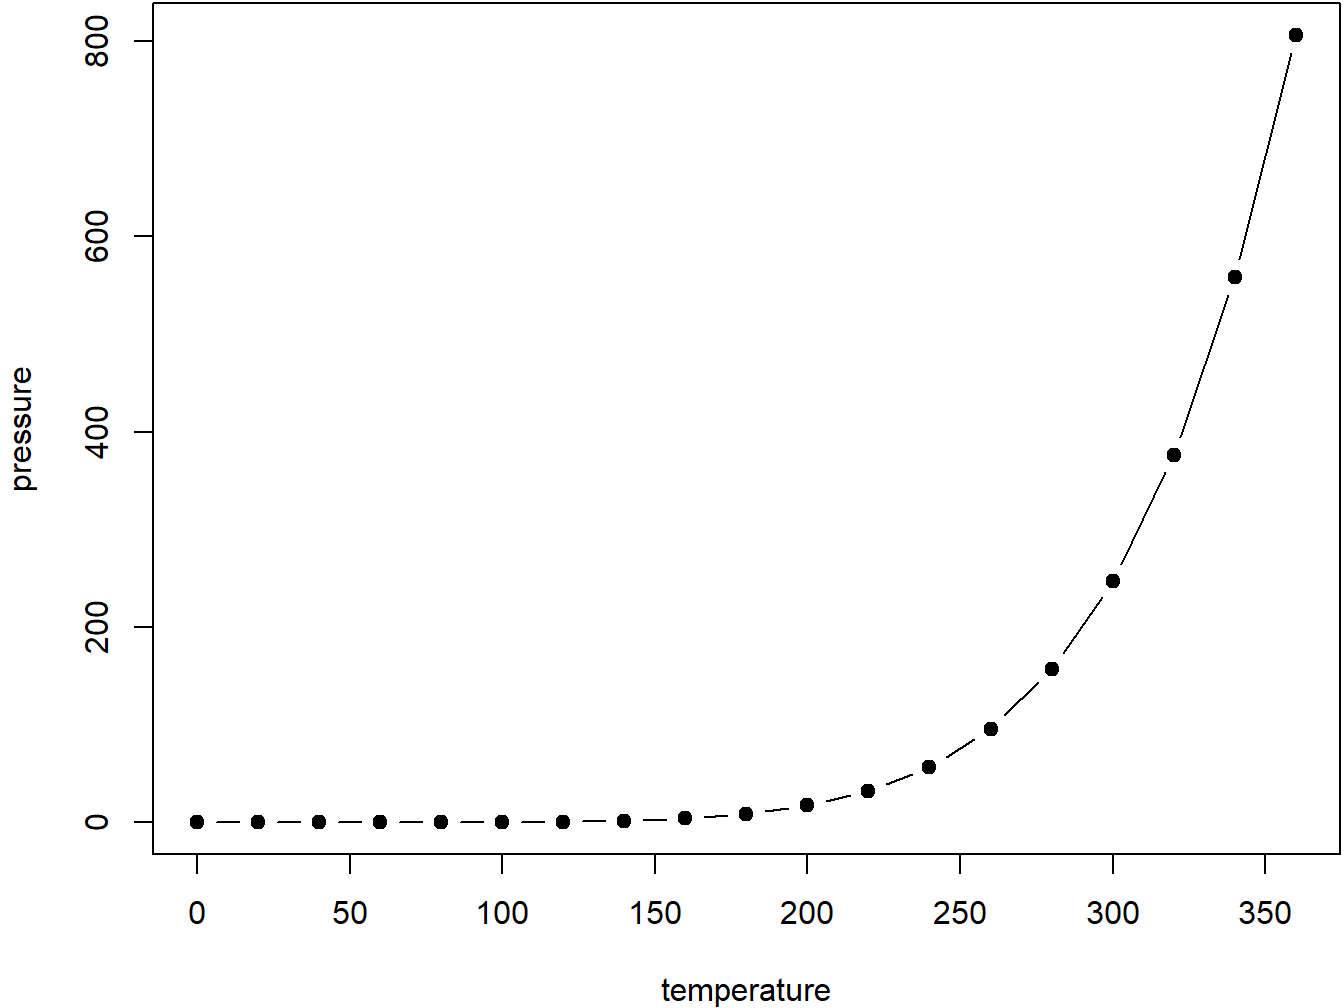
\includegraphics[width=0.8\linewidth]{data-analysis_files/figure-latex/nice-fig-1} 

}

\caption{Here is a nice figure!}\label{fig:nice-fig}
\end{figure}

Reference a figure by its code chunk label with the \texttt{fig:}
prefix, e.g., see Figure \ref{fig:nice-fig}. Similarly, you can
reference tables generated from \texttt{knitr::kable()}, e.g., see Table
\ref{tab:nice-tab}.

\begin{Shaded}
\begin{Highlighting}[]
\NormalTok{knitr}\OperatorTok{::}\KeywordTok{kable}\NormalTok{(}
  \KeywordTok{head}\NormalTok{(iris, }\DecValTok{20}\NormalTok{), }\DataTypeTok{caption =} \StringTok{'Here is a nice table!'}\NormalTok{,}
  \DataTypeTok{booktabs =} \OtherTok{TRUE}
\NormalTok{)}
\end{Highlighting}
\end{Shaded}

\begin{table}

\caption{\label{tab:nice-tab}Here is a nice table!}
\centering
\begin{tabular}[t]{rrrrl}
\toprule
Sepal.Length & Sepal.Width & Petal.Length & Petal.Width & Species\\
\midrule
5.1 & 3.5 & 1.4 & 0.2 & setosa\\
4.9 & 3.0 & 1.4 & 0.2 & setosa\\
4.7 & 3.2 & 1.3 & 0.2 & setosa\\
4.6 & 3.1 & 1.5 & 0.2 & setosa\\
5.0 & 3.6 & 1.4 & 0.2 & setosa\\
\addlinespace
5.4 & 3.9 & 1.7 & 0.4 & setosa\\
4.6 & 3.4 & 1.4 & 0.3 & setosa\\
5.0 & 3.4 & 1.5 & 0.2 & setosa\\
4.4 & 2.9 & 1.4 & 0.2 & setosa\\
4.9 & 3.1 & 1.5 & 0.1 & setosa\\
\addlinespace
5.4 & 3.7 & 1.5 & 0.2 & setosa\\
4.8 & 3.4 & 1.6 & 0.2 & setosa\\
4.8 & 3.0 & 1.4 & 0.1 & setosa\\
4.3 & 3.0 & 1.1 & 0.1 & setosa\\
5.8 & 4.0 & 1.2 & 0.2 & setosa\\
\addlinespace
5.7 & 4.4 & 1.5 & 0.4 & setosa\\
5.4 & 3.9 & 1.3 & 0.4 & setosa\\
5.1 & 3.5 & 1.4 & 0.3 & setosa\\
5.7 & 3.8 & 1.7 & 0.3 & setosa\\
5.1 & 3.8 & 1.5 & 0.3 & setosa\\
\bottomrule
\end{tabular}
\end{table}

You can write citations, too. For example, we are using the
\textbf{bookdown} package \citep{R-bookdown} in this sample book, which
was built on top of R Markdown and \textbf{knitr} \citep{xie2015}.

\begin{center}\rule{0.5\linewidth}{\linethickness}\end{center}

\hypertarget{rrstudio}{%
\section{R语言与RStudio}\label{rrstudio}}

\hypertarget{shiny}{%
\section{Shiny应用}\label{shiny}}

\section{调用其它语言程序}

\textbf{Powered by - Copyright® Intellectual Property Rights of
\href{http://www.scibrokes.com}{Scibrokes®}個人の経営企業}

\hypertarget{analytics}{%
\chapter{数据分析}\label{analytics}}

\section{读存数据}

\subsection{本地文件}

\subsection{外来文件}

\section{采集网络数据}

\subsection{普通采集}

\hypertarget{api}{%
\subsection{API接口}\label{api}}

\hypertarget{web-driver}{%
\subsection{Web Driver}\label{web-driver}}

\section{数据处理}

\subsection{文字与数字}

\subsection{数据框与矩阵}

\subsection{列表与嵌套数据}

\hypertarget{2.3}{%
\section{第2.3章:数据分析程序包}\label{2.3}}

\begin{center}\rule{0.5\linewidth}{\linethickness}\end{center}

\textbf{Powered by - Copyright® Intellectual Property Rights of
\href{http://www.scibrokes.com}{Scibrokes®}個人の経営企業}

\hypertarget{stats}{%
\chapter{统计模式}\label{stats}}

\section{基本统计学}

\subsection{线性模型}

\subsection{广义型线性模型}

\subsection{最优模型选择}

\section{高级统计学}

\subsection{极大似然估计}

\subsection{蒙地卡罗}

\subsection{马尔可夫链}

\subsection{隐马尔可夫链}

\subsection{贝叶斯分析}

\section{统计学程序包}

\begin{center}\rule{0.5\linewidth}{\linethickness}\end{center}

\textbf{Powered by - Copyright® Intellectual Property Rights of
\href{http://www.scibrokes.com}{Scibrokes®}個人の経営企業}

\hypertarget{finance}{%
\chapter{金融交易}\label{finance}}

\section{金融交易}

\subsection{金融交易介绍}

\subsection{金融数据}

\subsection{金融交易统计模型介绍}

\section{单变量统计模型}

\hypertarget{lassoelasticnetridge}{%
\subsection{LASSO、ElasticNet、RIDGE模型}\label{lassoelasticnetridge}}

\hypertarget{arima}{%
\subsection{Arima模型}\label{arima}}

\subsection{指数平滑法}

\hypertarget{garch}{%
\subsection{GARCH模型}\label{garch}}

\section{多变量统计模型}

\hypertarget{garch-1}{%
\subsection{GARCH模型}\label{garch-1}}

\hypertarget{section}{%
\subsection{}\label{section}}

\section{高频率交易模型}

\hypertarget{midas}{%
\subsection{MIDAS模型}\label{midas}}

\hypertarget{midas-garch}{%
\subsection{MIDAS-GARCH}\label{midas-garch}}

\hypertarget{garch-2}{%
\subsection{GARCH模型}\label{garch-2}}

\section{其它统计模型}

\hypertarget{levy-process}{%
\subsection{Levy Process}\label{levy-process}}

\hypertarget{wavelet-tranforms}{%
\subsection{Wavelet Tranforms}\label{wavelet-tranforms}}

\section{投资管理}

\subsection{投资风险管理}

\subsection{基金管理}

\subsection{多元基金管理}

\subsection{基金评估}

\section{金融交易程序包}

\begin{center}\rule{0.5\linewidth}{\linethickness}\end{center}

\textbf{Powered by - Copyright® Intellectual Property Rights of
\href{http://www.scibrokes.com}{Scibrokes®}個人の経営企業}

\hypertarget{sportsbook}{%
\chapter{体彩交易}\label{sportsbook}}

\section{体彩交易}

\subsection{体彩交易介绍}

\subsection{体彩数据}

\subsection{体彩交易统计模型介绍}

\section{足球赔率建模}

\subsection{单变量泊松模型}

\subsection{多变量泊松模型}

\hypertarget{logistic}{%
\subsection{Logistic模型}\label{logistic}}

\hypertarget{section-1}{%
\subsection{}\label{section-1}}

\section{足彩投注模型}

\subsection{普通投注模型}

\subsection{凯利投注模型}

\hypertarget{ohlcgarch}{%
\subsection{OHLC与GARCH应用}\label{ohlcgarch}}

\hypertarget{-1}{%
\section{投资管理}\label{-1}}

\section{体彩交易程序包}

\begin{center}\rule{0.5\linewidth}{\linethickness}\end{center}

\textbf{Powered by - Copyright® Intellectual Property Rights of
\href{http://www.scibrokes.com}{Scibrokes®}個人の経営企業}

\hypertarget{lottery}{%
\chapter{彩票、轮盘、老虎机与宾果}\label{lottery}}

\section{彩票分析与预测}

\subsection{数据与统计建模}

\subsection{投注模式与回酬}

\section{轮盘分析与预测}

\hypertarget{-1}{%
\subsection{数据与统计建模}\label{-1}}

\hypertarget{-1}{%
\subsection{投注模式与回酬}\label{-1}}

\section{老虎机分析与预测}

\hypertarget{-2}{%
\subsection{数据与统计建模}\label{-2}}

\hypertarget{-2}{%
\subsection{投注模式与回酬}\label{-2}}

\section{宾果分析与预测}

\hypertarget{-3}{%
\subsection{数据与统计建模}\label{-3}}

\hypertarget{-3}{%
\subsection{投注模式与回酬}\label{-3}}

\begin{center}\rule{0.5\linewidth}{\linethickness}\end{center}

\textbf{Powered by - Copyright® Intellectual Property Rights of
\href{http://www.scibrokes.com}{Scibrokes®}個人の経営企業}

\hypertarget{hft}{%
\chapter{高效率编程}\label{hft}}

\section{高效数据处理}

\begin{itemize}
\tightlist
\item
  \href{https://stackoverflow.com/questions/28447014/the-fastest-way-to-convert-numeric-to-character-in-r}{The
  fastest way to convert numeric to character in R}
\item
  \href{http://www.fstpackage.org/}{The \texttt{fst} package}
\item
  \href{https://d.cosx.org/d/420148-splitstackshape}{\texttt{splitstackshape}程序包}
\item
  \href{http://www.johnmyleswhite.com/notebook/2011/10/31/using-sparse-matrices-in-r/}{Using
  Sparse Matrices in R}
\item
  \href{https://appsilon.com/fast-data-loading-from-files-to-r/}{Fast
  data loading from files to R}
\end{itemize}

\section{高效统计建模}

\begin{itemize}
\tightlist
\item
  \href{http://rpubs.com/englianhu/binary-Q1FiGJRGARCH}{binary.com
  面试试题 I - GARCH模型中的ARIMA(p,d,q)参数最优化}
\end{itemize}

\hypertarget{r}{%
\section{高效率与高级R语言参考书}\label{r}}

\begin{itemize}
\tightlist
\item
  \href{https://csgillespie.github.io/efficientR/}{Efficient R
  programming}
\item
  \href{http://adv-r.had.co.nz}{Advanced R}
\end{itemize}

\begin{center}\rule{0.5\linewidth}{\linethickness}\end{center}

\textbf{Powered by - Copyright® Intellectual Property Rights of
\href{http://www.scibrokes.com}{Scibrokes®}個人の経営企業}

\hypertarget{fund}{%
\chapter{基金与投资者管理模型}\label{fund}}

\section{多元化基金管理}

\subsection{多元化基金评估}

\hypertarget{section-2}{%
\subsection{}\label{section-2}}

\section{投资者管理}

\subsection{投资者资金流动统计建模}

\hypertarget{section-3}{%
\subsection{}\label{section-3}}

\begin{center}\rule{0.5\linewidth}{\linethickness}\end{center}

\textbf{Powered by - Copyright® Intellectual Property Rights of
\href{http://www.scibrokes.com}{Scibrokes®}個人の経営企業}

\hypertarget{algorithm}{%
\chapter{程序交易}\label{algorithm}}

\section{交易自动化}

\subsection{数据连接自动化}

\subsection{统计运算自动化}

\subsection{基金评估自动化}

\subsection{客户管理自动化}

\section{多客户管理}

\subsection{多投资者}

\subsection{绩效管理}

\hypertarget{section-4}{%
\section{}\label{section-4}}

\begin{enumerate}
\def\labelenumi{\arabic{enumi}.}
\tightlist
\item
  \href{https://www.r-bloggers.com/calculating-the-house-edge-of-a-slot-machine-with-r/}{Calculating
  the house edge of a slot machine, with R}\footnote{\href{http://giorasimchoni.com/2017/05/06/2017-05-06-don-t-drink-and-gamble/}{DON'T
    DRINK AND GAMBLE:Analyzing and Simulating a Slot Machine - So You
    Don't Have To} and
    \href{https://www.schneier.com/blog/archives/2017/02/predicting_a_sl.html}{Predicting
    a Slot Machine's PRNG}}
\item
  \href{https://www.wired.com/2017/02/russians-engineer-brilliant-slot-machine-cheat-casinos-no-fix/}{Russians
  Engineer a Brilliant Slot Machine Cheat-and Casinos Have No Fix}
\item
  \href{https://srdas.github.io/MLBook}{Data Science: Theories, Models,
  Algorithms, and Analytics}
\item
  \href{github.com/englianhu/binary.com-interview-question}{Job
  Application - Quantitative Analyst}
\item
  \href{https://github.com/scibrokes/real-time-fxcm}{Real Time FXCM}
\item
  \href{https://github.com/scibrokes/Rmodel}{Rmodel}
\item
  \href{https://github.com/scibrokes/odds-modelling-and-testing-inefficiency-of-sports-bookmakers}{Odds
  Modelling and Testing Inefficiency of Sports Bookmakers}
\end{enumerate}

\begin{center}\rule{0.5\linewidth}{\linethickness}\end{center}

\textbf{Powered by - Copyright® Intellectual Property Rights of
\href{http://www.scibrokes.com}{Scibrokes®}個人の経営企業}

\bibliography{book.bib,packages.bib}


\end{document}
